\documentclass[11pt]{article}

\usepackage{comment}
\usepackage{wrapfig}
\usepackage{url}
\usepackage{color}
\usepackage{marvosym}
\usepackage{enumerate}
\usepackage{subfig}
\usepackage{amsmath}
\usepackage{amssymb}
\usepackage{hyperref}
\usepackage{tikz}
\usepackage{pgfplots}

\usepackage{caption}
\usepackage{graphicx}

\oddsidemargin 0mm
\evensidemargin 5mm
\topmargin -20mm
\textheight 240mm
\textwidth 160mm


\setlength{\parskip}{.5cm plus4mm minus3mm}

\def\ci{\perp\!\!\!\perp}

\newcommand{\vw}{{\bf w}}
\newcommand{\vx}{{\bf x}}
\newcommand{\vy}{{\bf y}}
\newcommand{\vxi}{{\bf x}_i}
\newcommand{\yi}{y_i}
\newcommand{\vxj}{{\bf x}_j}
\newcommand{\vxn}{{\bf x}_n}
\newcommand{\yj}{y_j}
\newcommand{\ai}{\alpha_i}
\newcommand{\aj}{\alpha_j}
\newcommand{\X}{{\bf X}}
\newcommand{\Y}{{\bf Y}}
\newcommand{\vz}{{\bf z}}
\newcommand{\msigma}{{\bf \Sigma}}
\newcommand{\vmu}{{\bf \mu}}
\newcommand{\vmuk}{{\bf \mu}_k}
\newcommand{\msigmak}{{\bf \Sigma}_k}
\newcommand{\vmuj}{{\bf \mu}_j}
\newcommand{\msigmaj}{{\bf \Sigma}_j}
\newcommand{\pij}{\pi_j}
\newcommand{\pik}{\pi_k}
\newcommand{\D}{\mathcal{D}}
\newcommand{\el}{\mathcal{L}}
\newcommand{\N}{\mathcal{N}}
\newcommand{\vxij}{{\bf x}_{ij}}
\newcommand{\vt}{{\bf t}}
\newcommand{\yh}{\hat{y}}
\newcommand{\code}[1]{{\footnotesize \tt #1}}
\newcommand{\alphai}{\alpha_i}

% custom imports
\newif\iftfanswer
\newif\ifunanswered
\newcommand{\answertruefalse}[1][\unansweredtrue]{
\unansweredfalse
#1
\ifunanswered
    \underline{Unanswered}
\else
    \iftfanswer
        \textbf{True}
    \else
        \textbf{False}
\fi
}
\newcommand{\answertruefalseN}[1][-1]{
\ifnum#1<0
    \underline{Unanswered}
\else
    \ifnum#1=0
        \textbf{False}
    \else
        \textbf{True}
    \fi
\fi}
\newcommand{\tftrue}{\answertruefalseN[1]}
\newcommand{\tffalse}{\answertruefalseN[0]}
\newcommand{\tfunanswered}{\answertruefalseN[-1]}
\newcommand{\inputsolution}[1]{\underline{\bf Solution}:

\input{#1}
}
% \newcommand{\odv}[2]{\frac{d #1}{d#2}}
\newcommand{\odv}[3][1]{
    \ifnum #1 =1
        \frac{d #2}{d#3}
    \else
        \frac{d^{#1} #2}{d#3^{#1}}
    \fi
}

\newcommand{\pdv}[3][1]{
    \ifnum #1 = 1
        \frac{\partial #2}{\partial#3}
    \else
        \frac{\partial^{#1} #2}{\partial#3^{#1}}
    \fi
}
\newcommand{\indep}{\mathrel{\perp\mkern-10mu\perp}} % independence
\newcommand{\given}{~\vert~}
\newcommand{\condindep}[3]{(#1 \indep #2 \given #3)} % conditional independence
\newcommand{\expect}[1]{\mathbb{E}\left[#1\right]}
\newcommand{\likelihood}{\mathcal{L}}
\DeclareMathOperator{\relu}{ReLU}
\DeclareMathOperator{\argmax}{argmax}
\DeclareMathOperator{\argmin}{argmin}
\DeclareMathOperator{\sign}{sign}

\newcounter{questionnumber}
\stepcounter{questionnumber}

\newcommand{\questionnumber}{\noindent \arabic{questionnumber}\stepcounter{questionnumber})~~}
\newcommand{\truefalse}[1]{\questionnumber #1\\True~~~~~~~~False\\Explanation:\\ }

\pagestyle{myheadings}
\markboth{}{Fall 2021 CS 475-675 Machine Learning: Midterm 2}


\title{CS 475-675 Machine Learning: Midterm 2\\
\Large{Fall 2021}\\
150 points. }
\author{}
\date{}


\begin{document}
\large
\maketitle
\thispagestyle{headings}

\vspace{-.5in}
\noindent Name (print):
\underline{\makebox[5in][l]{Dimitri Lezcano}} \\

\noindent JHED:
\underline{\makebox[5in][l]{dlezcan1}}


 \vspace{3cm}
 If you think a question is unclear or multiple answers are reasonable, please write a brief explanation of your answer,
 to be safe. Also, show your work if you want wrong answers to have a chance at some credit: it lets us see how much you understood.

 This exam is open-book: permitted materials include textbooks, personal notes, lecture material, recitation material, past assignments, the course Piazza, and scholarly articles and papers. Other materials are otherwise not permitted. It is not permitted to discuss or share questions or solutions of this exam with any person, via any form of communication, other than the course instructors.  It is not permitted to solicit or use any solutions to past exams for this course.
 \vspace{1cm}

 \textbf{ Declaration:}

I have neither given nor received any unauthorized aid on this exam. In particular, I have not spoken to any other student about any part of this exam.
The work contained herein is wholly my own.  I understand that violation of these rules, including using an unauthorized aid, copying from another person,
or discussing this exam with another person in any way, may result in my receiving a 0 on this exam.
\begin{center}
\noindent\underline{\makebox[6in][l]{}}

 Signature ~~~~~~~~~~~~~~~~~~~~~~~~~~~~~~~~~~~~~~~~~~~~~~~~~Date


 \vspace{3cm}
 Good luck!
 \end{center}

\newpage

\section*{True/False (50 points)}
For each question, circle (or otherwise clearly indicate) either True or False.  Regardless of which answer you chose, explain why.\\
2 points for correct True/False answer, -2 points for incorrect True/False answer, 3 points for a correct explanation, 0 points for an incorrect explanation.\\

\truefalse{
Computing single variable marginals in a DAG model is always possible by treating it as a Markov random field model.
}
\begin{align*}
    J(\beta) &= (\mathbf{y}-\mathbf{X}\beta)^T(\mathbf{y}-\mathbf{X}\beta)+\lambda\sum_i\beta_i^2 \\
    &= (\mathbf{y}^T-\beta^T\mathbf{X}^T)(\mathbf{y}-\mathbf{X}\beta)+\lambda\sum_i\beta_i^2 \\
    &= \mathbf{y}^T\mathbf{y}-\mathbf{y}^T\mathbf{X}\beta - \beta^T\mathbf{X}^T\mathbf{y}^T+\beta^T\mathbf{X}^T\mathbf{X}\beta+\lambda\sum_i\beta_i^2 \\
    &= \mathbf{y}^T\mathbf{y}-2\mathbf{y}^T\mathbf{X}\beta+\beta^T\mathbf{X}^T\mathbf{X}\beta+\lambda\sum_i\beta_i^2
\end{align*}
To minimize $J(\beta)$, we set $\frac{\partial J(\beta)}{\partial \beta} = 0$
\begin{align*}
    \frac{\partial J(\beta)}{\partial \beta} &=-2\mathbf{X}^T\mathbf{y} + 2\mathbf{X}^T\mathbf{X}\beta + 2\lambda \beta = 0 \\
    \mathbf{X}^T\mathbf{X}\beta + \lambda\mathbf{I}\beta &= \mathbf{X}^T\mathbf{y} \\
    (\mathbf{X}^T\mathbf{X} + \lambda\mathbf{I})\beta &= \mathbf{X}^T\mathbf{y} \\
    \beta &= (\mathbf{X}^T\mathbf{X} + \lambda\mathbf{I})^{-1}\mathbf{X}^T\mathbf{y}
\end{align*}

\vspace{0.5cm}

\truefalse{A DAG model is always observationally equivalent to a Markov random field model.}
\begin{align*}
p(p|f\cap not\; c)&=\frac{p(f\cap not\; c|p)\times p(p)}{p(f\cap not\; c)} \\
&=\frac{p(f|p)\times p(not \; c|p)\times p(p)}{p(f)-p(f \cap c)} \\
&=\frac{p(f|p)\times (1- p(c|p))\times p(p)}{p(f)-p(f \cap c)} \\
&=\frac{(0.5)\times (1-0.7)\times (0.05)}{(0.2-0.08)}=\frac{0.0075}{0.12}=0.0625
\end{align*}

\vspace{0.5cm}
% \newpage

\truefalse{Consider the following predictor trained from a dataset $[D]$ with features $\vec{X}$ and outcomes $Y$.  First, a $k$-means clustering algorithm is
trained using $k$ clusters, and treatment both $\vec{X}$ and $Y$ as ``features'' when computing the centroid distance.  Second, when a new data point
$\vec{X}_{\text{new}}$ is to be classifier, the predictor finds the closest of the $k$ centroids, and takes the majority vote among outcomes $Y$ in all points in that centroid.
This predictor is an example of a $k$-nearest neighbor algorithm.}
\begin{align*}
    p(\lambda |x) &\propto p(x|\lambda)p(\lambda) \\
    &\propto \lambda^ne^{-\lambda \sum_i x_i} \lambda^{\alpha -1}e^{-\beta \lambda} \\
    &\propto e^{-\lambda(\sum_ix_i-\beta)}\lambda^{n+\alpha-1} \\
    p(\lambda |x) &\propto Gamma(\alpha^*, \beta^*), where \; \alpha^* = \alpha +n \; and \; \beta^* =\sum_ix_i+\beta
\end{align*}



\vspace{0.5cm}

\truefalse{The GES Algorithm will always run in polynomial time in the size of the graph $k$ and the size of the data $n$.}
% \newcommand{\odv}[2]{\frac{d #1}{d#2}}
\newcommand{\odv}[3][1]{
    \ifnum #1 =1
        \frac{d #2}{d#3}
    \else
        \frac{d^{#1} #2}{d#3^{#1}}
    \fi
}

\newcommand{\pdv}[3][1]{
    \ifnum #1 = 1
        \frac{\partial #2}{\partial#3}
    \else
        \frac{\partial^{#1} #2}{\partial#3^{#1}}
    \fi
}
\begin{enumerate}[(i) ]
    \item $a_1 = -1 + 6 - 2 = 3$, $h_1 = 3$, $\yh = h_1 + 2 x_1 = 3 - 2 = 1$
    
    
    \item $\hat{y} = ReLU(w_1 x_1 + w_2 x_2 + w_3 x_3) + 2 x_1$
    
    
    \item The gradients of $l$ w.r.t $w_i$ is given by 
    $$
    \pdv{l}{w_i} = \pdv{l}{\yh}\pdv{\yh}{w_i} = -(y - \yh)\pdv{\yh}{w_i} = 
    \begin{cases}
    -(y-\yh) x_i, & w_1 x_1 + w_2 x_2 + w_3 x_3 > 0\\
    0, &\text{otherwise}
    \end{cases}
    $$
    We find that $\yh = ReLU(-1 + 6 + 2) - 2 = 5$. So $(y - \yh) = -1 - 5 = 6$.
    Therefore
    $$
    \left.\pdv{l}{w_1} = -6 (-1) = 6 ~\right|~
    \left.\pdv{l}{w_2} = -6 (-3) = 18 ~\right|~
    \pdv{l}{w_3} = -6 (-2) = 12
    $$
    
    
    \item In each case, we find that the update will follow the negative of the gradient direction and the update here $\Delta w_i \propto -\pdv{l}{w_i} < 0 ~\forall i = 1,2,3$, so each parameter will decrease.
    
    
    \item $\pdv{l}{v_1} = \pdv{l}{\yh}\pdv{\yh}{v_1} = -(y-\yh)x_1 = -6(-1) = 6$ and $\pdv{l}{v_2} = \pdv{l}{\yh}\pdv{\yh}{v_2} = -(y-\yh)h_1 = -6(7) = -42$. $v_{i,new} = v_i - \eta \pdv{l}{v_i}$, so we have $v_{1,new} = 2 - \frac{1}{2}(6) = -1$ and $v_{2,new} = 1 - \frac{1}{2}(-42) = 22$.
    
    
\end{enumerate}

\newpage

\truefalse{Two different undirected graphs (on the same set of vertices) correspond to different Markov random field models.}
\newcommand{\Graph}{\mathcal{G}}
\tftrue 

Suppose that $\Graph_1 = (V, E_1)$ and $\Graph_2 = (V, E_2)$ are different undirected graphs. Then (WLOG) $\exists$ at least a single pair $v_1, v_2 \in V$ s.t. $(v_1, v_2) \in E_1 \cap E_2'$. Therefore, since the graphs are MRFs, we can write the distributions of each of these graphs as
$$
p_{\Graph_i}(\vec{v}) = \frac{1}{Z} \prod_{v \in V} \phi(v) \prod_{(v_j, v_k) \in E_i} \phi(v_j, v_k).
$$

Note that $p_{\Graph_1} \neq p_{\Graph_2} \iff \exists p_{\Graph_1}(\vec{v})/p_{\Graph_1}(\vec{v}) \neq 1 $. So consider $p_{\Graph_1}(\vec{v})/p_{\Graph_2}(\vec{v})$
\begin{align*}
    \frac{p_{\Graph_1}(\vec{v})}{p_{\Graph_2}(\vec{v})} &= \frac{\frac{1}{Z} \prod_{v \in V} \phi(v) \prod_{(v_j, v_k) \in E_1} \phi(v_j, v_k)}{\frac{1}{Z} \prod_{v \in V} \phi(v) \prod_{(v_j, v_k) \in E_2} \phi(v_j, v_k)}\\
        &= \frac{\prod_{(v_j, v_k) \in E_1} \phi(v_j, v_k)}{\prod_{(v_j, v_k) \in E_2} \phi(v_j, v_k)}\\
        &= \frac{\prod_{(v_j, v_k) \in E_1\cap E_2'} \phi(v_j, v_k)}{\prod_{(v_j, v_k) \in E_2\cap E_1'} \phi(v_j, v_k)} ~\text{which is at least}\\
        &= \phi(v_1, v_2) \frac{\prod_{(v_j, v_k) \in E_1\cap E_2'\setminus(v_1, v_2)} \phi(v_j, v_k)}{\prod_{(v_j, v_k) \in E_2\cap E_1'\setminus(v_1, v_2)} \phi(v_j, v_k)} \neq 1 \because \phi(v_1, v_2) \neq 1 ~\text{generally}
\end{align*}
Therefore, two different MRFs results in distributions that are not equivalent. Furthermore, we have that in $\Graph_1$, ($v_1 \indep $ non-neighbors $\given v_2$ and other neighbors), but in $\Graph_2$, ($v_1 \indep$ non-neighbors $\given$ neighbors that don't include $v_2$). This results in a different independence which yields a different distribution.


\vspace{0.5cm}

\truefalse{$\mathbb{E}[Y^{(1)} \mid \vec{X}]$ is a function of the observed data distribution $p(Y,X,R_Y)$ if $Y$ is MAR given $\vec{X}$.
}
\tftrue

For each class $Y_l$ (say $l = 1, \dots, k$), define a perceptron with parameters $\beta_l$ such that 
$f_l(x) = \sign(\beta_l^T x)$ (including bias term in dot product) be the decision rule for $x$ to be classified as $Y_l$ or not $Y_l$. So here, we have $k$ perceptron classifiers, $f_l$, that determines whether each is either in a specific class or not. Since all of the classes are linearly separable, the class $Y_l$ is linearly separable with not $Y_l$ classes. So we train each perceptron to discriminate what is $Y_l$ and what is not $Y_l$ for $l = 1, \dots, k$, since these classes are linearly separable with what is $Y_l$ and what is not $Y_l$. 

\newpage

\truefalse{LDA can be used as a clustering algorithm.}
\tftrue 

Naive Bayes assumes $X_i \ci X_1, \dots, X_{i-1}, X_{i+1}, \dots, X_k \given Y ~\forall i = 1, \dots, k$. Take a graphical model, $\mathcal{G}$ where $Y$ is the root node and $X_i$ are all children of $Y$. In other words $\mathcal{G} = (\mathcal{V}, \mathcal{E})$ where $\mathcal{V} = \{ X_1, \dots, X_k, Y \}$ are the vertices and $\mathcal{E} = \{ (X_i, Y) \given  i = 1, \dots, k \}$ are the pair-wise edges of $\mathcal{G}$. Therefore, the maximal cliques of this graph are all of size 2 and we have the independences, $X_i \ci X_1, \dots, X_{i-1}, X_{i+1}, \dots, X_k \given Y ~\forall i = 1, \dots, k$, the same independence as Naive Bayes. Therefore by Hammersley-Clifford theorem, Naive Bayes factorizes w.r.t $\mathcal{G} \iff$ Naive Bayes obeys the global and local markov properties $\iff$ Naive Bayes is an MRF. 

% \emph{I think: Go through MRF properties}

\vspace{0.5cm}

\truefalse{Value iteration will always converge to the true \emph{value function} in a finite number of steps.}
\tffalse

Value iteration will always converge to the true value function in an infinite number of steps. We are not guaranteed convergence of a finite number of steps.

\newpage

\truefalse{The Newton-Raphson algorithm is a special case of gradient descent.}
\tftrue 

The goal for an SVM is to maximize the margin between two classes. Therefore, in order to calculate a margin, at the minimum, it will need one vector from each class that are the closest to the (linear) decision boundary to define the margin. Otherwise, the margin may not be maximized should the SVM only have one support vector (i.e. maximum between a single support vector is $\infty$).

\vspace{0.5cm}

\truefalse{Super learner will do better than any single predictor in its library, as sample size goes to infinity.}
\tffalse

\underline{Projection pursuit models}:  $M$ different linear combinations of features $\beta_m^T \vec{x}$ to learn a complex non-linear link functions and add the results
$$
f(\vec{x}) = \sum_{m=1}^M g_m(\beta_m^T \vec{x})
$$
for a set of \emph{unrestricted} $g_m(\cdot)$.

Here, logistic regression is actually a restricted moment model which learns $f(\vec{x}) = g(\vec{x}; \beta)$ where $g$ is \emph{fixed}, not unrestricted. Therefore, we have that logisitc regression is NOT a projection pursuit model.

\vspace{0.5cm}

\pagebreak

\section*{Multiple Part Questions (100 points).}

\questionnumber {\bf Message Passing (25 points)}
Consider the DAG below.
\vspace{-0.5cm}
\begin{center}
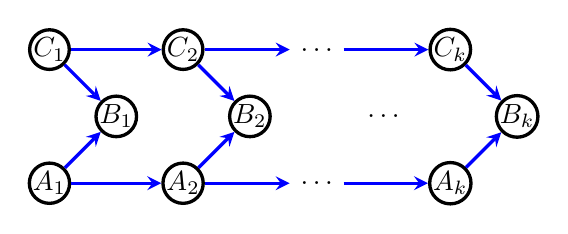
\begin{tikzpicture}[>=stealth, node distance=1.2cm]
    \tikzstyle{format} = [draw, very thick, circle, minimum size=5.0mm,
	inner sep=0pt]

	\begin{scope}
		\path[->, very thick]
			node[format] (A1) {$A_1$}
			node[format, above right of=A1] (B1) {$B_1$}
			node[format, above left of=B1] (C1) {$C_1$}
			
			node[format, below right of=B1] (A2) {$A_2$}
			
			node[format, above right of=A2] (B2) {$B_2$}
			node[format, above left of=B2] (C2) {$C_2$}

			node[below right of=B2] (d1) {$\ldots$}
			node[above right of=d1] (d2) {$\ldots$}
			node[above left of=d2] (d3) {$\ldots$}

			node[format, below right of=d2] (Ak) {$A_k$}
			node[format, above right of=Ak] (Bk) {$B_k$}
			node[format, above left of=Bk] (Ck) {$C_k$}

			(Ck) edge[blue] (Bk)
			(Ak) edge[blue] (Bk)
			
			(d1) edge[blue] (Ak)
			(d3) edge[blue] (Ck)

			(C2) edge[blue] (d3)
			(A2) edge[blue] (d1)

			(A1) edge[blue] (B1)

			(A2) edge[blue] (B2)

			(C1) edge[blue] (B1)
			
			(A1) edge[blue] (A2)
			(C1) edge[blue] (C2)
			(C2) edge[blue] (B2)
		;
	\end{scope}
\end{tikzpicture}
\end{center}
\vspace{-0.5cm}

\begin{itemize}

\item[(i)] What is the moralized and triangulated undirected graph corresponding to this DAG?  Since the DAG has repeating structure, feel free to only draw the first few "slices" of the graph.

\inputsolution{solutions/problem11/i}

\vspace{0.5cm}

\item[(ii)] Construct a clique tree from the graph in (i).  Again, since the clique tree has repeating structure, feel free to only draw enough of it so it's clear what the repeated structure is.

\inputsolution{solutions/problem11/ii}

\vspace{0.5cm}

\pagebreak

\item[(iii)] Do you expect message passing applied to the graph in (i) to run in polynomial time in $k$?  Explain.

\inputsolution{solutions/problem11/iii}

\vspace{0.5cm}

\end{itemize}

\newpage

\questionnumber {\bf Reinforcement Learning (25 points)}

Consider a reinforcement learning problem with states $s_0, s_1$, and two actions $a_0,a_1$.
We know the following:
{\small
\begin{align*}
p(s^{(t+1)} = s_1 \mid s^{(t)} = s_0, a_0) = 0.1; \hspace{0.2cm} p(s^{(t+1)} = s_1 \mid s^{(t)} = s_0, a_1) = 0.7\\
p(s^{(t+1)} = s_0 \mid s^{(t)} = s_1, a_1) = 0.8; \hspace{0.2cm} p(s^{(t+1)} = s_0 \mid s^{(t)} = s_1, a_0) = 0.2\\
R_{a_0}(s_0, s_1) = 1; \hspace{0.2cm} R_{a_1}(s_0, s_1) = -1, R = 0\text{ for all other state transitions and actions.}
\end{align*}
}
and let the discount factor be $\gamma = 0.5$.

\begin{itemize}
\item[(i)] What is $V^{(1)}(s_0)$ and $V^{(1)}(s_1)$ (value functions for states $s_0,s_1$ after a single loop of the value iteration algorithm)?  Show your work!

\inputsolution{solutions/problem12/i}

\vspace{0.5cm}

\item[(ii)] Without performing an explicit calculation, what do you think is the optimal policy for this problem?  Explain.

\inputsolution{solutions/problem12/ii}

\vspace{0.5cm}

\pagebreak

\item[(iii)] Assume that we did not know the transition probabilities in the above Markov chain.  Suggest a modification to value iteration that would be able to handle
this case, while still converging to the value function at every state.

\inputsolution{solutions/problem12/iii}

\vspace{0.5cm}

\item[(iv)] Assume rewards were not fixed, but drawn from distributions:
$R_{a_0}(s_0, s_1)\sim f_1(a_0,s_0,s_1)$ and $R_{a_1}(s_0, s_1) \sim f_2(a_1,s_0,s_1)$.  Suggest a modification to value iteration that would be able to handle
this case, while still converging to the value function $V^*(s)$ at every state $s$, where the value function is now defined as
{\small
\begin{align*}
V^*(s) = \mathbb{E}[ R_{a = \pi^*(s)}(s, s^{(1)})] + \gamma \mathbb{E}[ V^*(s^{(1)}) ],
\end{align*}
}
where the expectation is taken both with respect to the state transition probabilities, and $f_1$ and $f_2$.

\inputsolution{solutions/problem12/iv}

\vspace{0.5cm}

\end{itemize}

\newpage

\questionnumber {\bf Prediction With Missing Features (25 points)}

Assume we want to learn parameters $\beta$ of a regression problem $\mathbb{E}[Y \mid \vec{X}^{(1)}]$  we wish to solve, such that $\vec{X}^{(1)} = \{ X^{(1)}_1, X^{(1)}_2 \}$ is a pair of real-valued features, where either feature could be missing in our data.  Recall that in missing data problems, $X_i = X^{(1)}_i$ if $R_i = 1$, and $X_i = ?$ otherwise.

Assume that
{\small
\begin{align*}
R_1 \ci R_2, X^{(1)}_1 \mid Y,X^{(1)}_2; \hspace{0.2cm}
R_2 \ci R_1, X^{(1)}_2 \mid Y,X^{(1)}_1.
\end{align*}
}

\begin{itemize}

\item[(i)] Is the model MCAR, MAR or MNAR?  Explain.

\inputsolution{solutions/problem13/i}

\vspace{0.5cm}

\item[(ii)] Use these assumptions, and the graphoid axioms to show that
$p(r_1, r_2 \mid x_{1}^{(1)}, x_{2}^{(1)}, y)$ is a function of the observed data distribution $p(y,x_1,x_2,r_1,r_2)$.

\inputsolution{solutions/problem13/ii}

\vspace{0.5cm}

\pagebreak

\item[(iii)] Noting that $p(y, x^{(1)}_1, x^{(1)}_2) = \frac{ p(y, x_1, x_2, r_1 = 1, r_2 = 1) }{ p(r_1 = 1,r_2 = 1 \mid x_1^{(1)},x_2^{(1)}, y)}$, show that
$p(y, x^{(1)}_1, x^{(1)}_2)$ is a function of the observed data distribution $p(y,x_1,x_2,r_1,r_2)$.

\inputsolution{solutions/problem13/iii}

\vspace{0.5cm}

\end{itemize}

\newpage

\questionnumber {\bf The Noisy-OR Classifier (25 points)}

\begin{itemize}

\item[(i)] Given a set of binary features $\vec{X} = \{ X_1, \ldots, X_k \}$ a \emph{noisy-or} model for the outcome $Y$ has the form
{\small
\begin{align*}
p(Y = 0 \mid x_1, \ldots, x_k) = p(Y = 0 \mid \tilde{x}_1, \ldots, \tilde{x}_k) \prod_{i=1}^k p(\tilde{x}_i \mid x_i),
\end{align*}
}
where $p(Y = 0 \mid \tilde{x}_1 = 0, \ldots, \tilde{x}_k = 0) = 1$ ($Y = 0$ with probability 1 if all $\tilde{x}_i$ are zero), and $p(Y = 1 \mid \tilde{x}_1, \ldots, \tilde{x}_k) = 1$ otherwise.
Here, every $\tilde{x}_i$ is a hidden variable, and the model is parameterized by probabilities $p(\tilde{x}_i = 0 \mid x_i = 1)$ and $p(\tilde{x}_i = 0 \mid x_i = 0)$, since:
{\small
\begin{align*}
p(Y = 0 \mid x_1, \ldots, x_k) &= \prod_{i=1}^k p(\tilde{x}_i = 0 \mid x_i),\\
p(Y = 1 \mid x_1, \ldots, x_k) &= 1 - \prod_{i=1}^k p(\tilde{x}_i = 0 \mid x_i),\\
\end{align*}
}
Write down the conditional likelihood function for this model.

\inputsolution{solutions/problem14/i}

\vspace{0.5cm}

\item[(ii)] Can this conditional likelihood be maximized in closed form?  If so, explain how.  If not, suggest an iterative procedure for maximizing it.

\inputsolution{solutions/problem14/ii}

\pagebreak

\item[(iii)] Assume any $X_i$ may be missing completely at random, and $Y$ is always observed.  Is it appropriate to maximize the conditional log likelihood using only rows where all variables are observed?  Explain.

\inputsolution{solutions/problem14/iii}

\vspace{0.5cm}

\item[(iv)] Assume the noisy-or model is the true model of the conditional density for $p(Y \mid \vec{X})$ obtained from the observed data distribution for our dataset $[D]$.
Will the classifier $\arg\max_y p(Y = y \mid X_1 = x_1, \ldots, X_k = x_k)$ minimize the Bayes risk?  Explain.

\inputsolution{solutions/problem14/iv}

\vspace{0.5cm}

\end{itemize}

\end{document}

